% Template by Falko Galperin <falko1@tzi.de>, 2022, V1.0
% Main styling of the template comes from the ClassicThesis package by André Miede.

% IMPORTANT POINTS BELOW:
% - Look at the options between "CONFIGURATION HERE" and "CONFIGURATION ENDS".
% - Abstract.tex contains the abstract (can be disabled).
% - Inhalt.tex contains the contents of your thesis.
% - Glossar.tex contains the glossary (can be disabled) and further options.

% Less important points:
% - You can compile a PDF using `make` and clean up unnecessary files 
%   using `make clean`. `make pdf` combines both.
% - CMYK color space will be used so that printers don't get confused.
% - Feel free to configure other parts outside of the section below too,
%   e.g. uncomment the list of tables if you want that.

%%% CONFIGURATION HERE %%%

% Enter information about your thesis here, adjust as necessary.
% I recommend keeping the `\xspace` at the end.
\newcommand{\myTitle}{System porting to mobile devices at the example of the SEE project\xspace}
\newcommand{\mySubtitle}{Master Thesis\xspace}
\newcommand{\myName}{Roman Gressler\xspace}
\newcommand{\myNumber}{3217822\xspace}
\newcommand{\myProf}{Prof.\ Dr.\ Rainer Koschke\xspace}
\newcommand{\myOtherProf}{Prof.\ Dr.\ Zwetachter\xspace}
\newcommand{\myDepartment}{Faculty 3 --- Mathematics and Computer Science\xspace}
\newcommand{\myDegree}{Computer Science\xspace}
\newcommand{\myDate}{\today}
\newcommand{\myVersion}{\classicthesis}

% Whether links should be colored.
\def\colorLinks{true}

% Color for citations.
\def\citeColor{Periwinkle}

% Color for URLs.
\def\urlColor{Cyan}

% The file in which your BibLaTeX sources reside.
% Remove this line to disable the bibliography.
\def\sourcesFile{sources.bib}

% If you won't use the glossary template, remove the following line.
% Otherwise, set this to the filename of the glossary LaTeX file.
\def\glossaryFile{Glossar.tex}

% If you don't want to have an abstract, remove the following line.
% Otherwise, set this to the filename of the LaTeX file containing the abstract.
\def\abstractFile{Abstract.tex}

% Despite the seemingly broad implications of this option, it'll simply include a 
% disclaimer for readers in case you don't want to use something 
% like the "Gendersternchen". Set it to 1 to enable this disclaimer.
\def\disableGender{0}

% Set this to 1 if you want to use \section for the highest level of headings.
% Otherwise, \chapter will be used.
% IMPORTANT NOTE: This template assumes this value will be 1.
% If you choose to set it to something other than 1, you'll need to
% adjust this template's usage of \section and change it to \chapter.
\def\disableChapter{1}

% These are ClassicThesis options. 
% Don't forget to set drafting=false for the final version.
% If you have pdflatex, I recommend eulermath=true, it looks a bit better in my opinion.
\PassOptionsToPackage{
  drafting=true,  % print version information on the bottom of the pages
  tocaligned=false, % the left column of the toc will be aligned (no indentation)
  dottedtoc=true,  % page numbers in ToC flushed right
  eulerchapternumbers=true, % use AMS Euler for chapter font (otherwise Palatino)
  linedheaders=false,  % chaper headers will have line above and beneath
  floatperchapter=true,  % numbering per chapter for all floats (i.e., Figure 1.1)
  eulermath=false,  % use Euler fonts for mathematical formulae (only with pdfLaTeX)
  beramono=true,    % toggle a different monospaced font (w/ bold)
  style=classicthesis % classicthesis, arsclassica
}{classicthesis}

%%% CONFIGURATION ENDS %%%
% (Of course, feel free to modify the rest of the below code too.)

% ClassicThesis causes these false positive warnings, hence we silence them.
\RequirePackage{silence} % :-\
    \WarningFilter{scrreprt}{Usage of package `titlesec'}
    \WarningFilter{titlesec}{Non standard sectioning command}

\documentclass[twoside,openright,titlepage,numbers=noenddot,%headlines,
               headinclude,footinclude,cleardoublepage=empty,abstract=on,
               BCOR=5mm,paper=a4,listof=totocnumbered]{scrreprt}
\usepackage[utf8]{inputenc}
\usepackage[T1]{fontenc}

\PassOptionsToPackage{hyphens}{url}

\usepackage[english]{babel}
\usepackage[dvipsnames,usenames,cmyk]{xcolor}
\usepackage{hyperref} 
\usepackage{xspace}
% \usepackage[style=alphabetic]{biblatex}
\usepackage[round]{natbib} % Literatur und Referenzen
\usepackage{bm}
\usepackage{dsfont}
\usepackage{sidenotes}
\usepackage{newpxtext}
\usepackage{epigraph}
\usepackage{etoolbox}
\usepackage{multicol}
\usepackage{graphicx}
\usepackage{wrapfig}
\usepackage{microtype}
% Note: If you enable this, you need the -shell-escape flag.
%\usepackage{minted}
%\usemintedstyle{friendly}
\usepackage{xifthen}
\usepackage{enumitem}
\usepackage{calc}
\usepackage{subfig}
\usepackage{amssymb}
\usepackage{scalerel}
\usepackage[noend]{algpseudocode}
\usepackage{algorithm}
\usepackage{xstring}

\usepackage[normalem]{ulem}
\setlength{\columnsep}{0,1cm}

\usepackage{classicthesis}
\usepackage{titlesec}

% Make headings a little more discernable.
\titleformat*{\chapter}{\LARGE\bfseries}
\titleformat*{\section}{\Large\bfseries}
\titleformat*{\subsection}{\large\bfseries}

\hypersetup{colorlinks=\colorLinks, citecolor=\citeColor, 
    urlcolor=\urlColor, linktocpage=true, bookmarksnumbered,
  pdftitle={\myTitle},%
  pdfauthor={\textcopyright\ \myName, University Bremen},%
  pdfsubject={\mySubtitle},%
  pdfcreator={pdfLaTeX},%
  pdfproducer={LaTeX with classicthesis and FG-V1.0}%
}

%\ifdef{\sourcesFile}{\addbibresource{\sourcesFile}}{}

% Allow " instead of "` and "'
\usepackage{csquotes}
\MakeOuterQuote{"}

% Uncomment this if you want textsc to be a little (x 1.15) bigger.
%\usepackage{letltxmacro,scalefnt}
%\newcommand{\bigtextsc}[1]{\textsc{\scalefont{1.15}#1}}

% Some custom commands:
% Proper spacing for "z.B."
\newcommand{\zB}{z.\,B.\xspace}
% Command for TODOs, use either \TODO or \TODO{Details}
\newcommand{\TODO}[1]{\textbf{\textcolor{red}{\ifthenelse{\isempty{#1}}{TODO!}{TODO: #1}}}\xspace}
% Properly color Axivion's name.
\newcommand{\Axivion}{\textsc{{\color{black}{A}}{\color{red}{x}}{\color{black}{ivion}}}}

\newcommand{\Regie}[1]{\textbf{Regie:} #1}
\newcommand{\Stil}[1]{\textbf{Stil:} #1}

% Improve caption fonts.
\setkomafont{caption}{\footnotesize\itshape}
\setkomafont{captionlabel}{\usekomafont{caption}}

% Import glossary if necessary.
\ifdef{\glossaryFile}{\input{\glossaryFile}}{}

\begin{document}

\title{\myTitle}
\subtitle{\mySubtitle}
\author{\myName}
\date{\myDate} 

\raggedbottom
\selectlanguage{english}
\captionsetup[subfigure]{justification=centering}

\pagestyle{plain}
\pagenumbering{roman}

\begin{titlepage}
    \begin{addmargin}[-1cm]{-3cm}
	\begin{center}
		\Huge
		\vspace*{1cm}
        \begingroup
            \myTitle \\ \bigskip
        \endgroup
		\LARGE
        \mySubtitle\\
		\vspace{3cm}
 		\Large
		\myName\\
		\vspace{6pt}
        Matriculation number: \myNumber\\
		\vspace{1cm}
		\myDate\\
		\vspace{2cm}
 		
\includegraphics[width=6cm]{unibremen}\\
 		\vspace{1cm}
 		\large
 		\myDepartment\\
		\myDegree\\
		\vspace{4cm}
		\large
		1. Supervisor: \myProf\\
		2. Supervisor: \myOtherProf\\
		\vspace{1.5cm}
	\end{center}
    \end{addmargin}
\end{titlepage}
\cleardoublepage{}

\ifdef{\abstractFile}{%
\pdfbookmark[1]{Zusammenfassung}{abstract}
\chapter*{Abstract}
\input{\abstractFile}
\cleardoublepage{}
}{}

\pdfbookmark[1]{Erklärung}{erklaerung}
\chapter*{Erklärung}\label{erklaerung}
Ich versichere, diese Arbeit --- sofern dies nicht explizit anders
gekennzeichnet wurde --- ohne fremde Hilfe angefertigt zu haben.  Ich
habe keine anderen als die angegebenen Quellen und Hilfsmittel
benutzt.  Alle Stellen, die wörtlich oder sinngemäß aus
Veröffentlichungen entnommen sind, sind als solche kenntlich gemacht.

\bigskip

\noindent\textit{Bremen, den \today}
\smallskip
\begin{flushright}
    \begin{tabular}{m{5cm}}
        \\ \hline
        \centering\myName \\
    \end{tabular}
\end{flushright}

\vfill

\cleardoublepage{}

\pdfbookmark[1]{Danksagung}{Danksagung}
\begingroup
\let\clearpage\relax
\let\cleardoublepage\relax
\let\cleardoublepage\relax
\chapter*{Danksagung}
\TODO{Danksagung hier.}


\ifdef{\disableGender}{%
\if\disableGender1
\vfill
\chapter*{Gender-Hinweis}
Aus Gründen der besseren Lesbarkeit wird auf die gleichzeitige
Verwendung der Sprachformen männlich, weiblich und divers verzichtet.
Sämtliche Personenbezeichnungen gelten gleichermaßen für alle
Geschlechter.

\vfill
\fi
}{}
\endgroup

\cleardoublepage

\pagestyle{scrheadings}

% Table of contents:
\pdfbookmark[1]{\contentsname}{tableofcontents}
\tableofcontents

\clearpage

\ifdef{\disableChapter}{
\if\disableChapter1
\let\subsubsection\subsection
\let\subsection\section
\let\section\chapter
\fi}{}

\cleardoublepage
\pagenumbering{arabic}

\section{Concept}
\label{section:concept}
In this section a concept of a mobile \gls{see} version will be presented. 
Therefore, a prototype will be created to point out the features that a mobile version of \gls{see} requires.

Prototypes are a common way to express the needs of a system. 
It is a low-cost way of planning an implementation, that can highlight challenges regarding constraints of a system early on.

Even though a prototype will never be able to show every aspect and need of a complex system, it should still help to answering questions like: 
How should the system feel? How should it be implemented, and what are the key features? \cite{houde1997prototypes} 

\gls{see} is meant to be used by multiple platforms such as desktop devices, mobile devices and virtual reality devices.
Each device has different interaction constrains. 
While a desktop user will control the player with mouse and keyboard a mobile user will interact with virtual joysticks on a touchscreen.
Selecting nodes of a \gls{city} will be done by clicking it with a mouse on desktop devices, while a mobile device will require a touch input.

\subsection{Interface}

In the following a paper prototype will be presented that marks out a concept for the mobile interface.
Since the field of mobile development is quite young there few guidelines regarding the design of mobile device interfaces.
A guideline that is widely accepted is problematic to find. \cite{renaud2017demarcating}, \cite{punchoojit2017usability}

Major differences to desktop environments are the screen size, forms of input and input feedback.
To assure as much space is used for the actual interaction of the app the menu should just take as much space as needed.
As a study has found out, a size of at least 8*8 mm is needed to reduce error rates selecting the right button. \cite{conradi2015optimal} \cite{parhi2006target}
TODO WEITER AUSFÜHREN
SHORTCUTS WIE STRG Z NICHT MÖGLICH
 \cite{adipat2005interface} 

Moving the player will be handled with virtual joysticks as seen in figure \ref{fig:joystick}.
The left joystick will move the player through the virtual room and the right will move the camera angle or in other word the direction the player looks at.
The joysticks are placed in the left and right corner and should just take as much space as needed to be handled comfortably.
This way the player is able to navigate through the virtual room with his/her thumps while still having enough space to work on the \gls{city}.

\begin{figure}[htb]
    \centering
    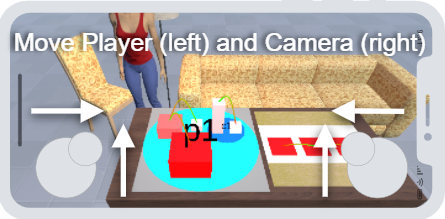
\includegraphics[width=1\textwidth]{Concept/img/joystick.png}
    \caption{Joysticks for moving in \gls{see}}\label{fig:joystick}
\end{figure}

The menu on the top left side seen in figure \ref{fig:quickbar} will be called "quickbar" further on. 
The quickbar can be minimized to safe screen space when not needed. 
The quickbar is designed to offer more general functions that are needed in various situations.
Because there are no shortcuts on mobile devices each function has to have a button to be activated.

The functions are redo and undo which will do an action undone again or revert an action.
Then there is a camera lock that will lock the players perspective to a certain \gls{city} so that the player can only move around the selected city and move closer or further away from it.
The next function is to rerotate a \gls{city}.
That means the \gls{city} that was last rotated will be set back to its initial state of rotation.
Last but not least there will be a button for recentering the city, which will work quite similar to the rerotate button and center the last moved \gls{city}.
The button on the right can be used to collapse or expand the quickbar.
\begin{figure}[htb]
    \centering
    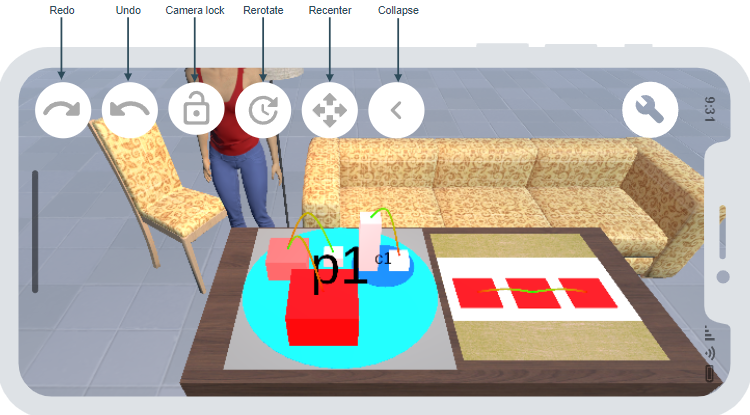
\includegraphics[width=1\textwidth]{Concept/img/quickbar.png}
    \caption{Quickbar for various interactions in \gls{see}}\label{fig:quickbar}
\end{figure}

On the top right side another menu will be placed that contains different interaction modes.
By clicking a button an interaction mode will be selected and moved to the top right corner.
Also, the menu will be collapsed and only the buttons regarding the selected interaction mode shall be shown.
By clicking the button on the top right again the menu shall expand and the other interaction modes shall be selectable.
The other buttons shall be kept in the same order to reduce confusion of the user.

The first interaction mode, seen in figure \ref{fig:select}, is for selecting nodes.
Nodes can be selected by being touched and deselected by being touched again.
There can be multiple nodes selected at once.
The hole selection can be deselected by clicking the deselect button next to the select interaction mode button.
Selected nodes shall be highlighted with a different node color and also display their name.

\begin{figure}[htb]
    \centering
    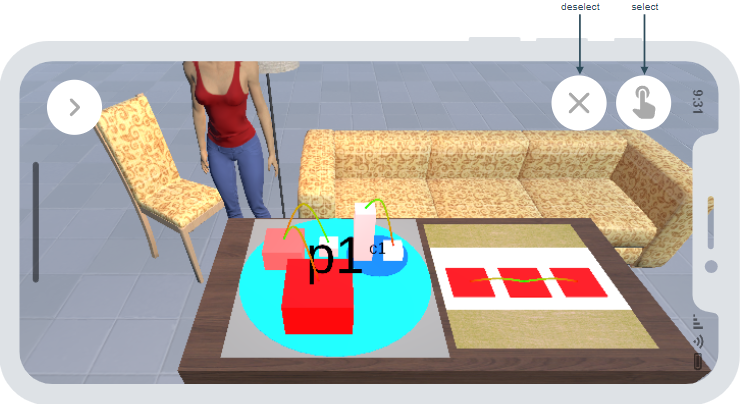
\includegraphics[width=1\textwidth]{Concept/img/menu1.png}
    \caption{Selection mode in \gls{see}}\label{fig:select}
\end{figure}

The second interaction mode, seen in figure \ref{fig:delete}, is for deleting node.
It does not need additional buttons.
Node will be deleted by being touched.-
Unlike in the desktop version there will not be a group deletion interaction because it would require an additional menu panel.
The added functionality would be minimal and selecting a group of nodes, confirming and finally deleting would require a handful more steps and would therefore most likely not be used.

\begin{figure}[htb]
    \centering
    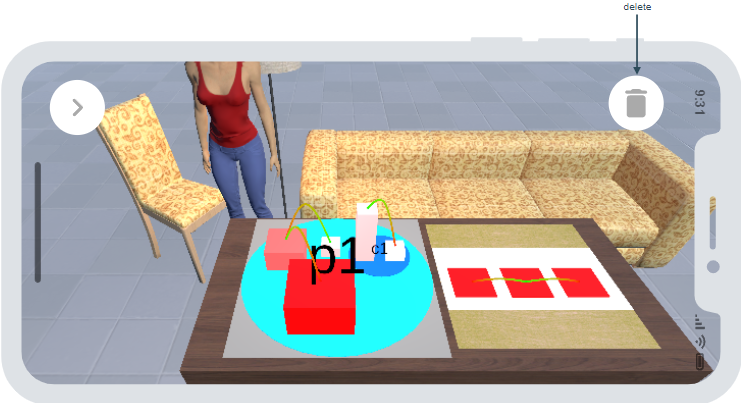
\includegraphics[width=1\textwidth]{Concept/img/menu2.png}
    \caption{Delete mode in \gls{see}}\label{fig:delete}
\end{figure}

The following interaction mode, seen in figure \ref{fig:nodes}, is dedicated to the nodes and edges of a \gls{city}.
Starting on with the "add node" button on the right.
When activated the user can create new node by clicking on a certain spot on the \gls{city} plane. 
The following button on the left is for adding edges.
By selecting two nodes a new edge will be created between them. 
Then, the button one further on the right is for editing nodes.
By touching a node a window will pop up that allows the user to edit the node by changing its name and its type.
Last but not least the button on the left-hand side will be used to scale nodes.
That means the node height and width can be adjusted by first selecting it via touch and then hold a corner and slide it further away from the node center to increase the size or slide it towards the center to decrease the size of the node.
Each button of the node interactions will be marked green after being pressed to indicate that it is active.

\begin{figure}[htb]
    \centering
    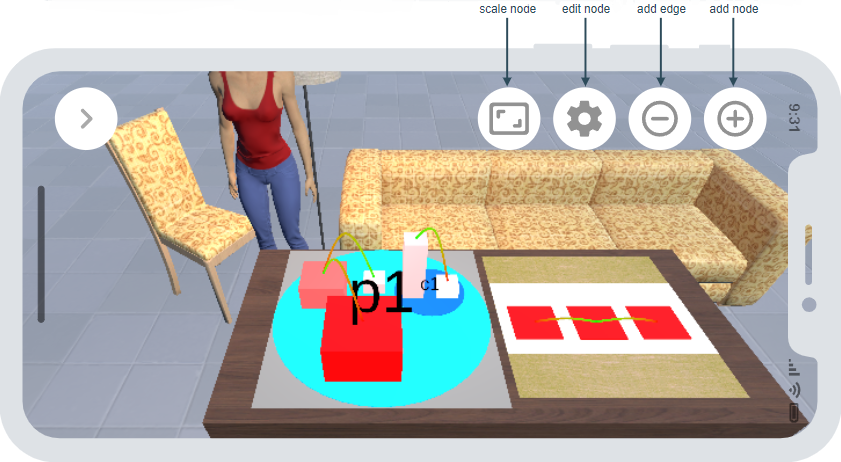
\includegraphics[width=1\textwidth]{Concept/img/menu3.png}
    \caption{Node interactions in \gls{see}}\label{fig:nodes}
\end{figure}

Then there will be a button for rotation interactions that can be seen in figure \ref{fig:rotate}.
Starting with the first activatable button that lets the user rotate the hole \gls{city} by touching any point on it and then sliding away from that point.
Similar to that there will be a button that lets the user rotate just a single node on the \gls{city}.
In addition to that there will be a button that activates the so-called "locked-rotation" mode.
While in "locked-rotation" mode the rotation of a node or \gls{city} will be done in eight predefined steps to a full rotation.
Each step will have the same 45° range.
The last button of this group will be for changing the center of the rotations. 
There are to options: the first option is a center of rotation in the middle of the \gls{city} and the second is in the middle of a node selection made with the interactions seen in figure \ref{fig:select}.
The second option can be activated by pressing the last button.

\begin{figure}[htb]
    \centering
    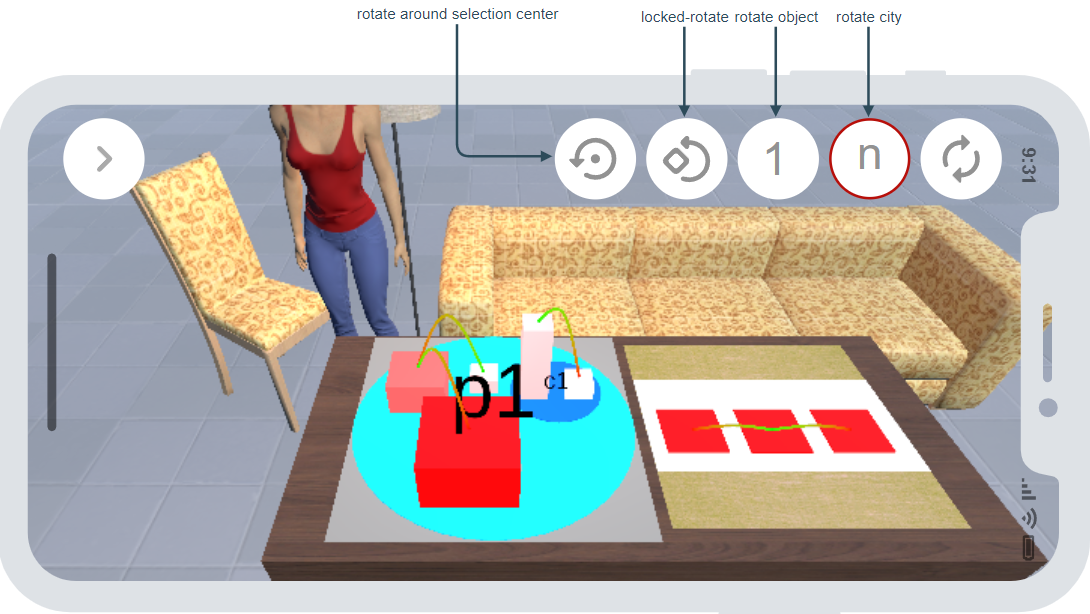
\includegraphics[width=1\textwidth]{Concept/img/menu4.png}
    \caption{Rotation mode in \gls{see}}\label{fig:rotate}
\end{figure}

The last interaction group, seen in figure \ref{fig:move}, is for moving the \gls{city} or a single node.
The move interactions are quite similar to the rotation interactions.
There will be a button to move a hole \gls{city} as well as a button to move only single nodes.
In addition to that there will be a button that restricts the movement of the \gls{city} or node to a predefined direction.
The directions will be again in 45° angles and objects can be moved on a straight line on that angle.
Moving a node or a \gls{city} can be achieved by touching and holding it and then moving it to the desired position.
\begin{figure}[htb]
    \centering
    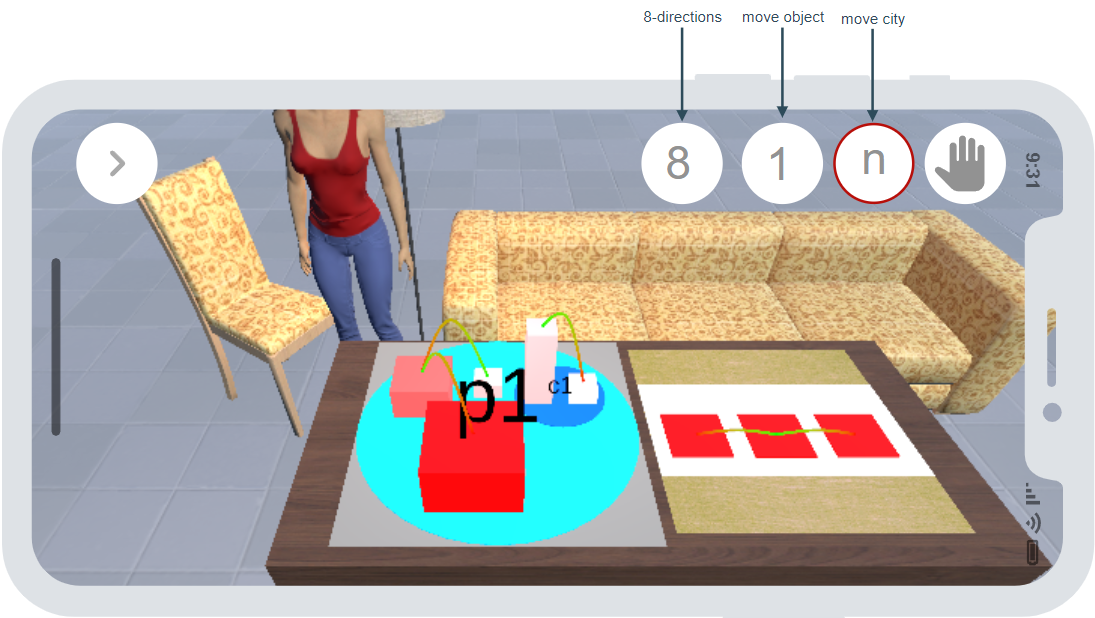
\includegraphics[width=1\textwidth]{Concept/img/menu5.png}
    \caption{Movement mode in \gls{see}}\label{fig:move}
\end{figure}

\subsection{Interaction}

Smartphones are quite limited in space and there are few input possibilities.
Unlike a desktop computer there is no mouse and there is no physical keyboard.
Smartphones use virtual keyboards but due to the restriction of screen space the keyboard is hidden most of the time.
Which would make keyboard shortcuts uncomfortable because the user has to open the keyboard first.
Therefore, smartphones need different ways of interaction such as touch gestures. 

Zooming in to a \gls{city} happens by scrolling on a desktop environment. 
The is no option to scroll on mobile devices, but there are at least two popular alternatives.
The first option would be to double tap on the \gls{city} to zoom in.
The double tap would zoom in, in predefined steps and after reaching a certain level of closeness it would trigger to zoom out again.
In \gls{see} zooming in, in predefined steps might not be precise enough because there could be a quite large \gls{city} or a rather small one.
Finding predefined steps that would fit every situation is rather hard.
Therefore, a second option by zooming in with a two finger gesture might be better. 
In this option the user uses two fingers and slides them towards each other to zoom in or slides the two fingers away from each other to zoom out.
This way there are no predefined steps necessary and zooming interactions can be done precisely.
\subsection{Requirements}
In the following a list of requirements will be given, which will specify in detail what the implementation of a mobile version has to take care of.
The list will be referred to multiple times in the upcoming realization part in chapter \ref{section:implementation}.
Requirements are essential for the planning phase as they give a good fundamental structure for the developer to rely on. \cite{Robertson2012,Stevens2005}
\begin{itemize}
    \item[{[R1]}] The application shall run on Android devices
    \item[{[R2]}] The application shall be controlled via touchscreen
    \begin{itemize}
        \item [{[R2.1]}] The player and camera shall be moved with virtual joysticks
        \item [{[R2.2]}] Needed shortcuts of the desktop version shall be handled with buttons
        \item [{[R2.3]}] Zooming shall be handled with a two finger gesture
    \end{itemize}
    \item[{[R3]}] The user shall be able to select a node of a \gls{city}
    \begin{itemize}
        \item [{[R3.1]}] After selecting the name of the node shall be shown
        \item [{[R3.2]}] The user shall be able to deselect single nodes or a group of nodes
    \end{itemize}
    \item[{[R4]}] The user shall be able to delete nodes
    \item[{[R5]}] The user shall be able to interact with nodes
    \begin{itemize}
        \item [{[R5.1]}] The user shall be able to add nodes
        \item [{[R5.2]}] The user shall be able to add edges
        \item [{[R5.3]}] The user shall be able to edit nodes
        \item [{[R5.4]}] The user shall be able to scale nodes
    \end{itemize}
    \item[{[R6]}] The user shall be able to rotate a \gls{city}
    \begin{itemize}
        \item[{[R6.1]}] The user shall be able to rotate a \gls{city} in 45° steps
        \item[{[R6.2]}] The user shall be able to rotate single objects
        \item[{[R6.3]}] The user shall be able to rotate around a center of selected nodes
        \item[{[R6.4]}] The user shall be able to undo the rotation
    \end{itemize}
    \item[{[R7]}] The user shall be able to move a \gls{city}
    \begin{itemize}
        \item[{[R7.1]}] The user shall be able to move single object of a \gls{city}
        \item[{[R7.2]}] The user shall be able to restore the \gls{city} initial position
        \item[{[R7.3]}] The user shall be able to move a \gls{city} or single node in predefined directions
    \end{itemize}
    \item[{[R8]}] The user shall be able to undo and redo actions
    \item[{[R9]}] The user shall be able to lock the camera to a selected \gls{city}
\end{itemize}
\section{Implementation}
\label{section:implementation}

This chapter will discuss the implementation of the mobile version of \gls{see}.
Starting with the mobile player implementation in section \ref{sec:player}.
Section \ref{sec:player_movement} will give insight on the player movement before section \ref{sec:menu} will discuss the mobile menu.
Next the implemented player action will be introduced in section \ref{sec:player_actions}.
This chapter will close with pointing out the requirements for an \gls{android} build and how they have been handled.
\subsection{Mobile Player}
\label{sec:player}
In this section the mobile player \gls{prefab} will be discussed. 
\gls{see} is supported on multiple platforms and with each platform having different requirements each platform needs to be divided.
Therefore, each platform gets its own player \gls{prefab}.
The mobile player prefab for the \gls{android} version of \gls{see} can be seen in figure \ref{fig:prefab}.

\begin{figure}[htb]
    \centering
    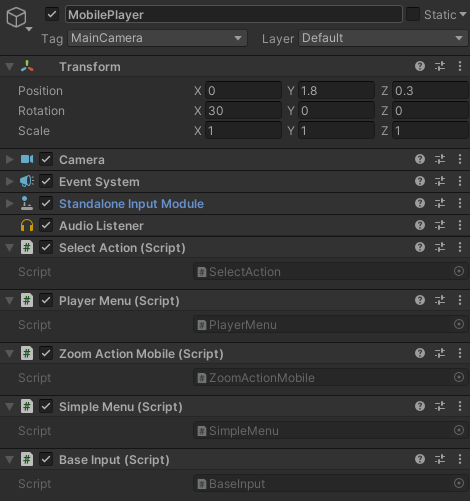
\includegraphics[width=0.8\textwidth]{Implementation/img/mobile_player.png}
    \caption{The mobile player \gls{prefab}}\label{fig:prefab}
\end{figure}

The \gls{prefab} consists of the basic parts provided by \gls{unity} \textit{Camera}, \textit{Event System}, \textit{Standalone Input Module} and \textit{Audio Listener}.
In addition to that the following custom scripts were added.
There is the \textit{SelectAction} and the \textit{ZoomActionMobile} script, which will both be discussed in section \ref{sec:player_actions}, and then there is the \textit{PLayerMenu} script, which creates the right menu based on the player type.
In this case the player type will be \enquote{mobile player} and the menu created (here \textit{SimpleMenu}) will be discussed in section \ref{sec:menu}.

\subsection{Player Movement}
\label{sec:player_movement}
After having creating a player, the player also has to be able to move.
Therefore, the \textit{MobilePlayerMovement} script got added.
The script handles the input by the joysticks seen in figure \ref{fig:joystick}.
To fulfill [R2.1] the player will be moved by using the left joystick and the player's perspective will be handled by the right joystick.

\begin{figure}[htb]
    \centering
    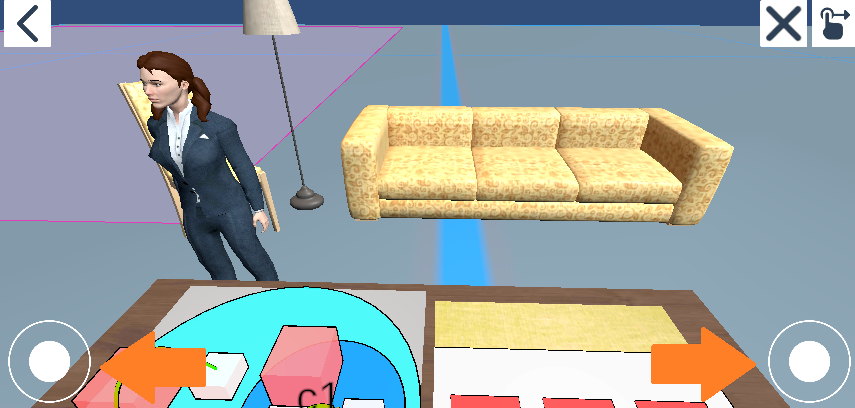
\includegraphics[width=1\textwidth]{Implementation/img/joysticks.png}
    \caption{The joysticks are for moving in the virtual room. The left joystick is for moving the player and the right one is for moving the player's perspective.}\label{fig:joystick}
\end{figure}

For the joystick \glspl{prefab} the \textit{Joystick Pack}\footnote{https://assetstore.unity.com/packages/tools/input-management/joystick-pack-107631\#description (last visited: 17.06.22, 15:21)} \gls{asset} is used.
It contains the design and basic logic for the joysticks.
A joystick returns a horizontal and a vertical value depending on how far the joystick is dragged into a direction.
The left joystick data can then be transformed into player movement as follows:
\begin{enumerate}
    \item Get the horizontal and vertical values from the joysticks
    \item Transform the values into a 3D vector
    \item Combine the values into a velocity vector
    \item Normalize the velocity vector for a smooth transition
    \item Transmit the velocity vector to the player position value
\end{enumerate}

The data of the right joystick shall move the player's perspective, which is implemented as a \gls{unity} camera.
The camera has a pitch angle and a yaw angle as illustrated in figure \ref{fig:camera}.
The angles of the camera will be adjusted with the input from the right joystick. 
For the angles of the player's perspective there is a range from 0° to 360° after reaching an end of this range the value will be transformed to the other end of the range.
In other words if the angle grows higher than 360° it starts at 0° again and if it gets lower than 0° it can go further down from 360°.
That way the player's perspective can move a full rotation.
\begin{figure}[htb]
    \centering
    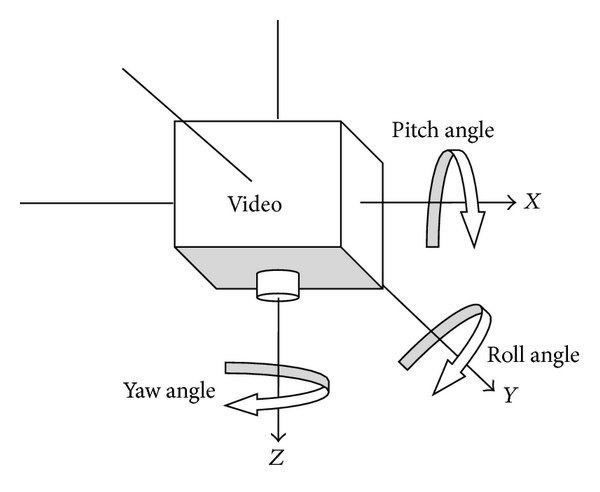
\includegraphics[width=1\textwidth]{Implementation/img/pitch_yaw.jpg}
    \caption{The angles of a camera by \cite{Zhang2014}}\label{fig:camera}
\end{figure}

\subsection{Mobile Menu}
\label{sec:menu}

The mobile menu is essential for the implementation since the input methods of a smartphone in an everyday usage are limited.
The desktop version uses many \glspl{shortcut}, which cannot be used in the mobile version.
These \glspl{shortcut} will replaced with buttons in the menu to fulfill requirement [R2.2].

\begin{figure}[htb]
    \centering
    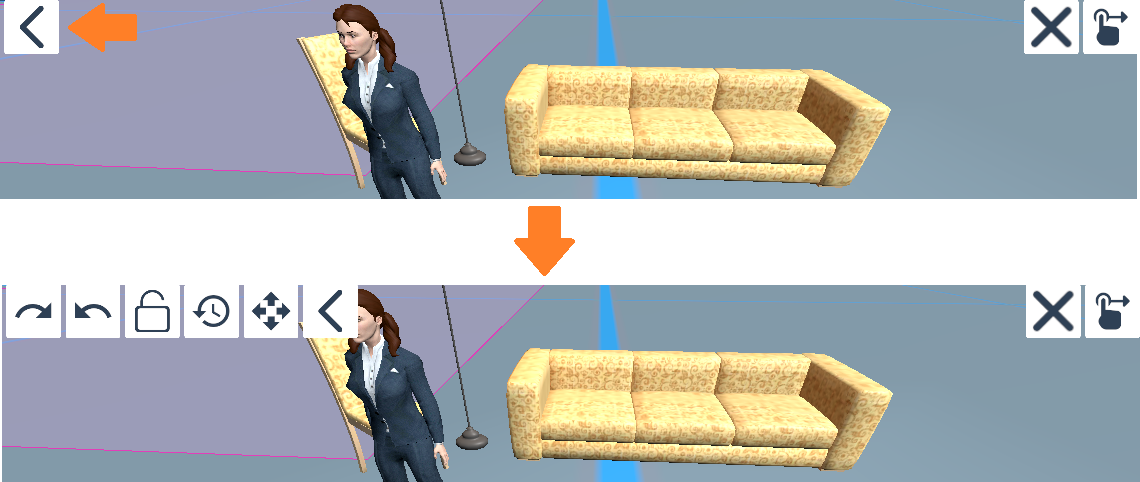
\includegraphics[width=1\textwidth]{Implementation/img/quickmenu.png}
    \caption{The \textit{quickbar} on the left top side of the mobile device. Pressing the button with an orange marked arrow will expand the menu.}\label{fig:quickmenu}
\end{figure}

The menu will be divided into to parts.
The first part, that was named \textit{quickbar} in section \ref{sec:interface}, will be responsible for all interactions that need to be available at all times.
The implemented \textit{quickbar} can be seen in figure \ref{fig:quickmenu}.
By pressing the button on the right end of the \textit{quickbar} the menu can be expanded and minimized to safe screen space when not needed.
The menu also contains buttons for redoing and undoing actions to fulfill requirement [R8].
In addition, that there is a button for a \enquote{locked-mode}.
Unfortunately the button is just a placeholder since the functionality to lock the players view to a city is not available in the desktop version at this time.
Therefore, requirement [R9] can not be completed at the time of this thesis. 

The other part of the menu can be seen in figure \ref{fig:interaction_menu}.
The menu is placed on the right side of the screen, and it contains all the player interactions.
This part of the menu is slightly more complex since the selected button moves to the top, while the other buttons shall remain their initial order.

\begin{figure}[htb]
    \centering
    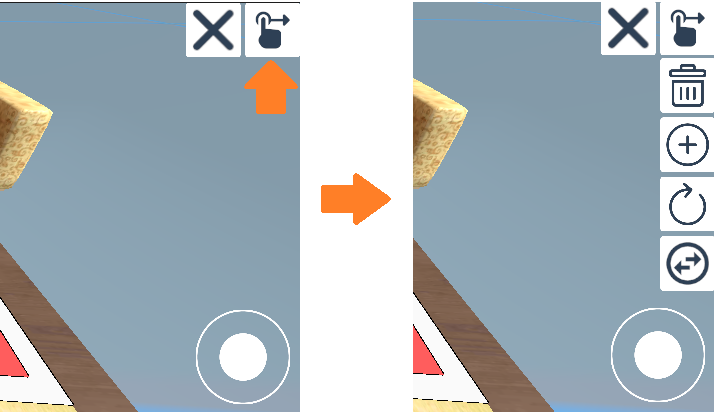
\includegraphics[width=1\textwidth]{Implementation/img/menu.png}
    \caption{The player interaction menu on the right top side of the mobile device. The button on the top right side indicate the active interaction mode. Pressing the same button also expands the menu.}\label{fig:interaction_menu}
\end{figure}

The implementation of the menu on the right is done in the following steps:
\begin{enumerate}
    \item All main buttons get an index
    \item When a button on the far right side gets clicked the index gets saved
    \item The button group with the selected index get shown on the top right side
    \item All other buttons get disabled
    \item By clicking the button on the top right again the other main buttons get reactivated 
    \item The order is as follows: selected index → index in ascending order
\end{enumerate} 
This way the selected interaction mode will always be in the top right corner, while the other buttons remain the same order.

\subsection{Player Actions}
\label{sec:player_actions}

One essential part of the implementation are the player actions. 
Almost all interactions a user can make in \gls{see} differ from the interactions in the desktop version.
In the following the implementation of all mobile player actions will be shortly discussed.

\subsubsection{Zooming}
To fulfill requirement [R2.3] zooming needs to be implemented.
The interaction of zooming in or out of a \gls{city} can be fundamental when working with a large \gls{city} because \glspl{node} become small and especially on a small mobile screen it becomes impossible to interact with those nodes via touch input. 
Therefore, the user has to zoom in to properly interact with the desired node.

Luckily the general zooming function is already implemented in \gls{see}.
The zooming method- requires a center point and a scale of how far the \gls{city} shall be zoomed in or out.
Zooming on a touchscreen will be done by dragging two fingers either towards or away from each other as visualized in figure \ref{fig:zooming}.

\begin{figure}[htb]
    \centering
    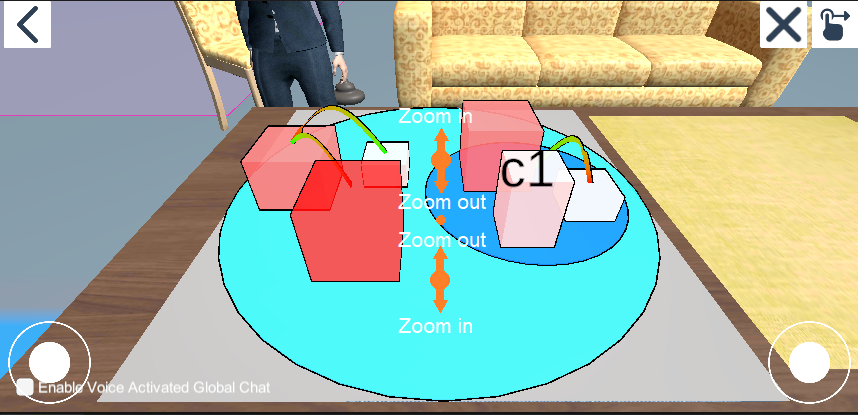
\includegraphics[width=1\textwidth]{Implementation/img/zoom.png}
    \caption{Dragging the two touch points towards each other will zoom out and dragging them away from each other will zoom in.}\label{fig:zooming}
\end{figure}

The implementation of the zooming interaction in done in the following steps: 
\begin{enumerate}
    \item Check if there are two touch inputs on the same \gls{city}. If both inputs are not on the same city zooming is not wanted and will not be activated.
    \item Compute the center of the two touch inputs
    \item Pass the center and dragging range of the two inputs to the zooming function
\end{enumerate}

Note that the direction of zooming has been inverted in the version used for the evaluation in chapter \ref{section:evaluation}.
This is because of the heavy demand by the subjects to invert the direction of zooming since it feel odd.

\subsubsection{Selecting and Deleting}
The interactions of selecting and deleting a \gls{node} or \gls{plane} are quite similar because the user selects or deletes an object by touching it.
The object get determined by a ray cast from the center of the touch position as discussed in section \ref{sec:ray}.

Since the selecting mode is always enabled except when the delete mode is active, the select button really does nothing except ensuring that no other interaction mode is active.
Keeping the selected objects active makes sense for the mobile version because the user cannot hover with a mouse to see the object names.
Therefore, the selection will be kept and not discarded by selecting a different object as in the desktop version.
The deselect button call the already implemented \textit{UnselectAll} method that empties a list of selected items.

To delete interaction works as already mentioned just like in the desktop version. 
The only difference is the type of input. 
Other than in the desktop version the mobile version only supports single deletions and not the deletion of multiple objects at once.
This is due to the limited space for the interactions menu and the results from a multi deletion can also be achieved with the single delete interaction.

The discussed implementation fulfills requirements [R3] and [R4].
\subsubsection{Node Interactions}
The node interactions consist of four types.
The active interaction is always highlighted in green as seen in figure \ref{fig:node}
\begin{figure}[htb]
    \centering
    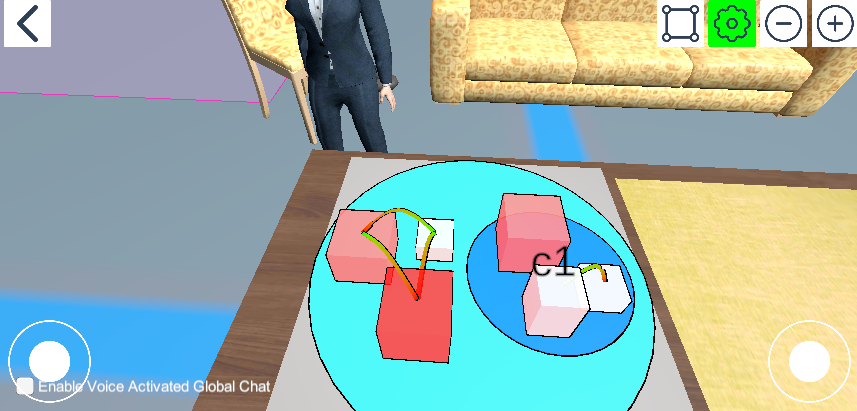
\includegraphics[width=1\textwidth]{Implementation/img/node.png}
    \caption{The node interactions menu. The active node interaction has a green button}\label{fig:node}
\end{figure}

The circled plus button stands for adding a \gls{node}.
Adding \glspl{node} is implemented in the following steps:
\begin{enumerate}
    \item Check if the device is an \gls{android} with a preprocessor tag
    \item Check if there is exactly on touch input
    \item Cast a ray and check if the collided object is of the type \enquote{Node} (\gls{see} does not distinguish between \gls{plane} and \gls{node} as a type)
    \item Create a \gls{node} ad that position with the already implemented \textit{AddChild} method of the class \textit{GameNodeAdder}
\end{enumerate}

The circled minus button is for adding an \gls{edge}.
The implementation is quite similar to the one for adding \glspl{node}.
In this case however the first and second \gls{gameObject} of type \enquote{\gls{node}} will be saved.
After there are two \glspl{gameObject} an \gls{edge} between those objects will be created.

Next in line is the gear button, which can be used for editing \glspl{node}.
The implementation here is almost the same as for the desktop version.
A \gls{node} or a \gls{plane} can be selected by touch and a window will open.
In that window attributes like the name can be changed.
Different from the desktop version is that a virtual keyboard will pop up to let the user type in a new name for example.

Last but not least there is the interaction of scaling a node left.
The implementation here was largely adopted from the desktop version, except again the input type is via touch.
In addition to that the dots that can be selected and dragged are larger in the mobile version (see figure \ref{fig:scale}) because otherwise it would be hard to hit them with a touch input.

\begin{figure}[htb]
    \centering
    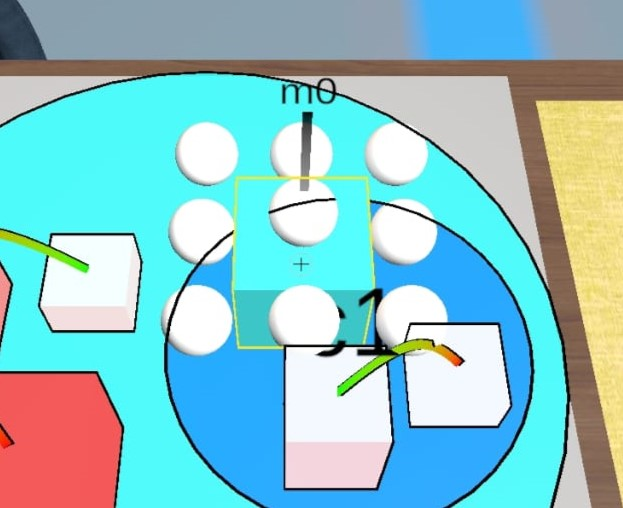
\includegraphics[width=0.7\textwidth]{Implementation/img/scale.jpeg}
    \caption{The node interactions menu. The active node interaction has a green button}\label{fig:scale}
\end{figure}

The listed implementations of the node interactions fulfill the requirements of [R5].

\subsubsection{Rotating}
To fulfil the requirements of [R6] rotating has to be adapted to the mobile version of \gls{see}.
The user can rotate the city either freely or in eight predefined steps.
Figure \ref{fig:rotate} shows a rotation in those eight predefined steps.
As it can be seen the \enquote{8} button is green which means that it is active.
The user can drag from a certain point on the \gls{city} towards a direction the \gls{city} shall be rotated to.

\begin{figure}[htb]
    \centering
    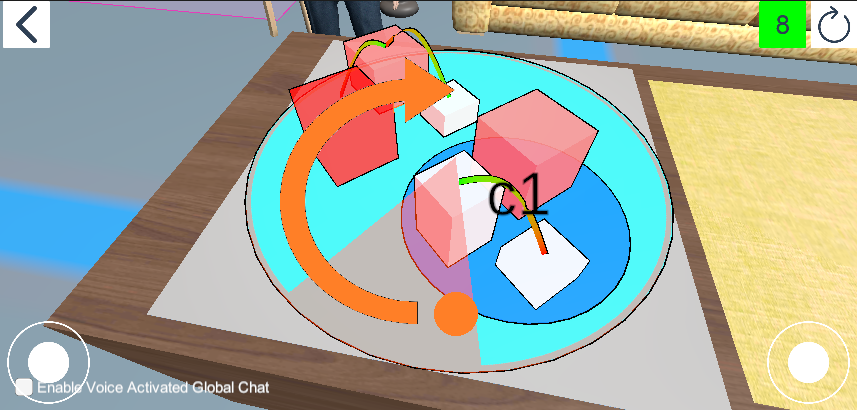
\includegraphics[width=1\textwidth]{Implementation/img/rotate.png}
    \caption{The \gls{city} can be rotated by for example touching the screen on the orange dot and dragging from there like the arrow indicates.}\label{fig:rotate}
\end{figure}

The implementation for the interaction of rotating is done in the following steps:
\begin{enumerate}
    \item Check if there is exactly one touch input on an object of the type \enquote{\gls{node}}.
    \item Check if the \enquote{8} button is active
    \item Calculate the new position of the \gls{city} just like in the desktop version of \gls{see}
\end{enumerate}
\subsubsection{Moving}
Last but not least the player action of moving a \gls{city} or object has to be implemented to fulfill the requirements of [R7].
The user can touch a certain point on a \gls{city} and drag it to move it as visualized in figure \ref{fig:move}.
The same can be done with any \gls{node} or \gls{plane} by activating the \enquote{1} button.
Same as for the rotate-interaction the user can also activate the \enquote{8} to move an object or city in one of eight predefined directions.
Also, by selecting the \enquote{1} or \enquote{8} button it will turn green to indicate that it is active.

\begin{figure}[htb]
    \centering
    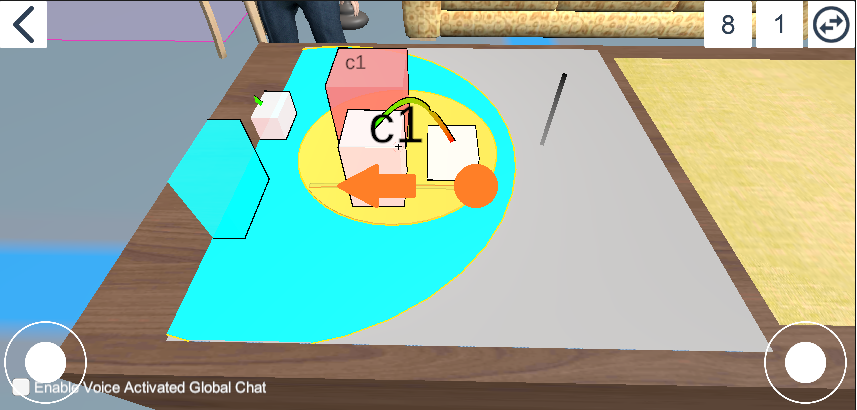
\includegraphics[width=1\textwidth]{Implementation/img/move.png}
    \caption{The \gls{city} can be moved by touching and dragging it to a desired direction.}\label{fig:left}
\end{figure}

The implementation is done similar to the one for the rotate-interaction. 
The only thing added here is the check whether the \enquote{1} button is active or not.

Not that for the rotate and move interactions the \enquote{n} buttons have been removed (see figure \ref{fig:rotate_proto} and figure \ref{fig:move}).
This is because these buttons are not needed since the initial mode when entering the interaction is already for the hole \gls{city}.
Also, the rotate object button and the rotate around selection center button have been removed. 
Rotating around a selection center will always be activated and can be deactivated by removing the selection of objects.
Rotating single objects is not intended as an interaction in \gls{see}.

\subsection{Android Build Requirements}
The last part of this chapter will discuss the requirements to build a version of \gls{see} on \gls{android} to fulfill the last requirement [R1].
In the following there will be a deeper look at the challenges porting \gls{see} to android devices brings. 


\subsubsection{Conditional Compilation}

\gls{see} uses as it is usual for a medium to large \gls{unity} project many \glspl{asset}.
Unfortunately not all \glspl{asset} support a \gls{android} implementation.
Therefore, the unsupported assets have to exchanged or excluded from the implementation.
Some unsupported \glspl{asset} are \textit{Valve} and \textit{UnityEngine.Windows.Speech}.
The \textit{Valve} \gls{asset} is required for the \gls{vr} implementation of \gls{see} and \textit{UnityEngine.Windows.Speech} is fundamental for the speech assistant \enquote{See}.
Since the \glspl{asset} are not supported but still needed in the project they need to be excluded. 

Unity offers a way to compile only partial code. 
Therefore, it uses the \textit{directives}\footnote{https://docs.unity3d.com/Manual/PlatformDependentCompilation.html (last visited: 21.06.2022, 1:27)} of the C\# language. 
These the hash character (\#) followed by \textit{if} or \textit{endif} to mark code areas with a condition.
\gls{unity} has platform scripting symbols like \textit{UNITY\_ANDROID} to set conditions for code areas to be compiled for a certain device or not.
The following code example shows how the technique is used in this project. 

\begin{minipage}{\linewidth}

\begin{lstlisting}[language=C]
using SupportedPackage
#if not UNITY_ANDROID
using NotSupportedForAndroidPackage
#endif 

    SomeClass
    {
    ...
    SomeSupportedPackageMethod()
    ...
    #if not UNITY_ANDROID
    SomeNotAvailableMethodForAndroid()
    #endif
    ...
    }
\end{lstlisting}

\end{minipage}

Examples like this can be found many times in the \gls{see} project. 
In addition to that there are some cases where the main code is exchanged whether the device is an \gls{android} or not.
For example the player actions discussed earlier in this chapter require touch input and can not use the hover effect of a mouse cursor on a mobile device.
Therefore, on mobile devices the touch input code will be used and on desktop devices the mouse hover code, but both code parts use the same methods and variables.
Having two separated classes would make up redundant code. 
On the other hand side excessive use of conditional compilation makes it harder to maintain code because it might have to be adjusted at multiple points for a single change.
This way part of the code could easily be forgotten and lead to bugs.

\subsubsection{File Loading}
One last challenge for the mobile implementation of \gls{see} was how files are handled in the project.
\gls{see} uses specify file space for \gls{unity} called \textit{StreamingAssets}\footnote{https://docs.unity3d.com/Manual/StreamingAssets.html (last visited: 21.06.22, 2:47)} to store for example the various states of an Evolution-\gls{city}.
An Evolution\gls{city} visualizes multiple states of development.
Only the first state is preloaded the other states are stored in the \textit{StreamingAssets} and are loaded at runtime. 
The problem however is that an \gls{android} application is packed into an \gls{jar}.
Files inside a \gls{jar} cannot be obtained without further ado.
To achieve access to files that are not initially loaded \textit{WebRequests}\footnote{https://docs.unity3d.com/ScriptReference/Networking.UnityWebRequest.html (last visited: 21.06.22, 3:13)} have to be used for an \gls{android} implementation. 
Therefore, once again the code needs to be divided and handled with conditional compilation.
This has to be done at every point in the code where files are obtained the common way with \textit{SystemIO} methods. 


\subsubsection{Restructuring}
\label{sec:restructure}
The disadvantage of conditional compilation is that it makes code harder to maintain as discussed earlier.
To minimize this disadvantage it was thought of restructuring the entire project to only have conditional compilation at a core component of \gls{see}.

The concept idea was to restructure the project in a way that from a core component all the different versions get initialized and only in that core component conditional compilation gets used.
All components would have abstract super classes that could be easily supplemented with assets that are not available for all platform.
The platform specific classes would then only be compiled for a certain platform build, since they are divided in the core class.

Unfortunately \gls{see} is already entangled and a restructuring in the described way above would take a high effort.
\gls{see} already has many components that depend on other part of \gls{see}. 
These parts however depend also on other parts of \gls{see}. 
Restructuring and setting a new order for the parts of see that support the idea of a core part of \gls{see} would take too much effort for this thesis and was therefore not implemented.
\section{Conclusion}
\label{section:conclusion}
...
\subsection{Outlook}
AR - \cite{santos2016guidelines}

\appendix

\ifdef{\glossaryFile}{
    % Print all glossaries here
    \printglossaries
}{}

% List of Figures.
\listoffigures

\vspace{8ex}

% List of Tables. Uncomment if you want to include.
%\listoftables

\vspace{8ex}

\Regie{Kontrolliere am Ende, ob alle bibliographischen Angaben
  vollständig sind.  Wird also die Zeitschrift oder Konferenz
  aufgeführt, in der ein Artikel veröffentlicht wurde?  Sind überall
  die Seitenangabe aufgeführt? Bei Verweisen auf Web-Seiten, ist
  überall angegeben, wann der letzte Zugriff darauf erfolgte? Sind
  Umlaute und andere Sonderzeichen korrekt in LaTeX beschrieben
  worden?}

% Finally, the bibliography.
\ifdef{\sourcesFile}{
\bibliographystyle{unsrtnat}
\bibliography{\sourcesFile}
%\printbibliography[heading=bibnumbered]
}{}

\end{document}
